\section{Java}

\begin{defi}{Servlet-Engine}
    Eine \emph{Servlet-Engine} enthält und verwaltet eigene Servlets über ihren gesamten Lebenszyklus.

    Sie bindet die Servlets über feste vorgegeben Interfaces ein und stellt die Dienste zum Empfangen von Anfragen und Senden von Antworten bereit.

    Somit bildet sie die Kommunikationsendpunkte für die Servlets, die über HTTP-URLs angesprochen werden können.
\end{defi}

\begin{defi}{Servlet}
    Ein \emph{Servlet} ist eine abgeleitete Java-Klasse, die von einem Container verwaltet wird und dynamische HTML-Inhalte generiert.

    Servlets haben keine \texttt{main}-Methode.
    Die programmtechnische Nutzung wird durch die Servlet-API gesteuert:
    \begin{itemize}
        \item \texttt{init}
        \item \texttt{service} oder \texttt{doGet} bzw. \texttt{doPost}
        \item \texttt{destroy}
    \end{itemize}

    Sie sind dauerhafte Prozesse, die zumeist auch über Anfragen hinweg existieren.

    Mehrere Anfragen existieren in der gleichen Instanz.

    Ein spezifisches Servlet unterliegt einem genau festgelegten Lebenszyklus:
    \begin{enumerate}
        \item Laden der \texttt{Servlet}-Klasse und instanziieren (on demand)
        \item Initialisieren des \texttt{Servlet}-Objekts
        \item Verarbeitung der verschiedenen Anfragen
        \item Entfernen des \texttt{Servlet}-Objekts
        \item Entladen der \texttt{Servlet}-Klasse
    \end{enumerate}

    Intern stehen drei Umgebungsvariablen zur Verfügung:
    \begin{itemize}
        \item \texttt{PATH\_INFO} bzw. \texttt{req.getPathInfo();}
        \item \texttt{REMOTE\_HOST} bzw. \texttt{req.getRemoteHost();}
        \item \texttt{QUERY\_STRING} bzw. \texttt{req.getQueryString();}
    \end{itemize}
\end{defi}

\begin{example}{Servlet}
    \begin{lstlisting}[language=Java]
        import java.io.*;
        import javax.servlet.*;
        import javax.servlet.http.*;

        public class PokemonServlet extends HttpServlet {
            public void init() { ... }
            public void destroy() { ... }

            public void doGet(HttpServletRequest req, HttpServletResponse res)
                throws IOException, ServletException {
                res.setContentType("text/html");
                PrintWriter out = response.getWriter();

                // Cookie
                Cookie cookie = new Cookie("lieblings_pokemon", "Glumanda");
                res.addCookie(cookie);

                // Session
                HttpSession session = request.getSession();
                session.setAttribute("lieblings_pokemon", "Glumanda");
                
                out.println(
                    "<html>\n" +
                    "<head>\n" +
                    "<title> Pokemon </title>\n" +
                    "</head>\n" +
                    "<body> Glumanda [4] </body>\n" +
                    "</html>\n"
                )
            }
        }
    \end{lstlisting}
\end{example}

\begin{defi}{Tomcat}
    \emph{Tomcat} ist eine vollständig in Java geschriebene Open-Source-Referenzimplementierung der Apache Foundation der Servlet-API.

    Es dient als leichtgewichtiger Servlet-Container, der z.B. keine Enterprise JavaBeans unterstützt.
\end{defi}

\begin{defi}{JSP}
    \emph{Java Server Pages (JSP)} kehren die Idee der Servlets \enquote{Java-Code generiert HTML} um in: \enquote{HTML-Seiten beinhalten Java-Code}.

    Die Anweisungen werden durch spezielle Tags gekennzeichnet.

    JSP-Seiten werden automatisch in Servlets übersetzt.
\end{defi}

\begin{bonus}{JSP-Elemente}
    Es gibt neben den HTML-Elementen drei wichtige \emph{JSP-Konstrukte}:
    \begin{itemize}
        \item \emph{Scripting-Elemente} bzw. \emph{Java-Fragmente}:
              \begin{itemize}
                  \item \texttt{pageContent}: Zugriff auf Objekte in den verschiedenen Gültigkeitsbereichen
                  \item \texttt{HttpServletRequest}
                  \item \texttt{session}: sitzungsorientierte Anwendung
                  \item \texttt{out}: Ausgabe
              \end{itemize}
        \item \emph{Direktiven}, die die Gesamtstruktur des Servlets kontrollieren:
              \begin{itemize}
                  \item \texttt{page} (Importieren einer Klasse)
                  \item \texttt{include} (Fügt weitere JSP-Datei ein)
                  \item \texttt{taglib} (Einführen eigener JSP-Tags)
              \end{itemize}
        \item \emph{Aktionen} bzw. \emph{Funktionalitäten} zur Laufzeit, die das Servlet beeinflussen:
              \begin{itemize}
                  \item \texttt{include} (Einfügen einer HTML- oder JSP-Seite zur Laufzeit)
                  \item \texttt{forward} (Anfragen und Antworten an eine andere JSP-Seite übergeben)
              \end{itemize}
    \end{itemize}
\end{bonus}

\begin{example}{JSP}
    \begin{lstlisting}[language=Java, alsolanguage=html5]
        <%@ page contentType="text/html" %>
        <!DOCTYPE html>
        <html>
        <head> <title> Pokemon </title> </head>
        <body>
            <p> <%= String.toUpperCase("Glumanda"); %> </p>
            <% out.println("Glumanda > Bisasam!"); %>
        </body>
        </html>
    \end{lstlisting}
\end{example}

\begin{bonus}{Wiederholung Model-View-Controller}
    \emph{Model-View-Controller}  ist ein Muster zur Unterteilung einer Software in die drei Komponenten \emph{Model}, \emph{View} und \emph{Controller}.
    Das Muster kann sowohl als Architekturmuster als auch als Entwurfsmuster eingesetzt werden.

    Ziel des Musters ist ein flexibler Programmentwurf, der eine spätere Änderung oder Erweiterung erleichtert und eine Wiederverwendbarkeit der einzelnen Komponenten ermöglicht.
    Die Umsetzungen nutzen dasselbe Model, nur Controller und View müssen dabei jeweils neu implementiert werden.

    Das \emph{Model} enthält Daten, die von der Präsentation dargestellt werden.
    Es ist von View und Controller unabhängig.

    Die \emph{View} ist für die Darstellung der Daten des Models und die Realisierung der Benutzerinteraktionen zuständig.
    Sie kennt das Model, dessen Daten sie präsentiert, ist aber nicht für die Verarbeitung dieser Daten zuständig.
    Des Weiteren ist sie von dem Controller unabhängig.

    Der \emph{Controller} verwaltet die View und das Model.
    Er wird von der View über Benutzerinteraktionen informiert, wertet diese aus und nimmt daraufhin Anpassungen an der View sowie Änderungen an den Daten im Model vor.

    \begin{center}
        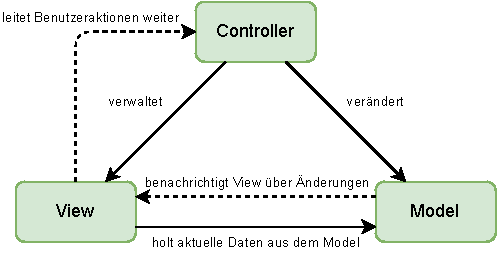
\includegraphics[width=0.7\textwidth]{includes/figures/defi_mvc.pdf}
    \end{center}
\end{bonus}

\begin{defi}{Model View Controller (Java)}
    \begin{center}
        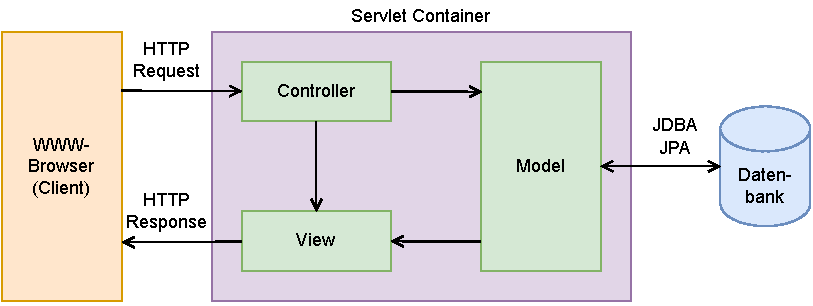
\includegraphics[width=0.75\textwidth]{includes/figures/defi_model_view_controller.pdf}
    \end{center}

    \begin{itemize}
        \item Model:
              \begin{itemize}
                  \item Realisation zumeist mittels JavaBeans
                  \item JavaBeans enthalten die eigentliche Programmlogik
                  \item JavaBeans berechnen die Ergebnisse und speichern Zustände
                  \item JavaBeans sind unabhängig von der Webschnittstelle
              \end{itemize}
        \item View:
              \begin{itemize}
                  \item Nutzung von JSP-Seiten
                  \item Anzeige der Ergebnisse
                  \item Ziel: Möglichst wenig Java Code
              \end{itemize}
        \item Controller:
              \begin{itemize}
                  \item Programmieren eines Servlets
                  \item Einlesen und Überprüfen der übergeben Parameter
                  \item Aufrufen der eigentlichen Programmlogik im Model
                  \item Weitergabe des Ergebnisses an die passende View
              \end{itemize}
    \end{itemize}
\end{defi}

\begin{defi}{JavaBeans}
    JavaBeans sind Software-Komponenten für die Programmiersprache Java.
    JavaBeans entwickelten sich aus der Notwendigkeit heraus, GUI-Klassen (AWT, Swing) einfach zu instanziieren.

    JavaBeans werden auch als Container zur Datenübertragung verwendet.

    Daher zeichnen sich alle JavaBeans durch folgende Eigenschaften aus:
    \begin{itemize}
        \item Öffentlicher parameterloser Konstruktor
        \item Serialisierbarkeit (Serializable)
        \item Öffentliche Zugriffsmethoden (Public Getters/Setters)
    \end{itemize}

    Mit \emph{Enterprise JavaBeans} können wichtige Konzepte für Unternehmensanwendungen, z. B. Transaktions-, Namens- oder Sicherheitsdienste, umgesetzt werden, die für die Geschäftslogik einer Anwendung nötig sind.
\end{defi}